\documentclass[a4paper,12pt]{report}
\usepackage{thesis}


% The value for \thesistitle should be the title of the thesis in a single line.
\renewcommand{\thesistitle}{
Visibility Driven Focus+Context Visualization of Multimodal Volume Data
}

% The value for \authorname should be the name of the student as per the
% administrative records. Add your roll number here within paranthesis.
\renewcommand{\authorname}{Srinivas R. Vaidya (MT2013152)}

% The value for \mydegree should be 
% 1: for M.Tech., 
% 2: for M.S. by research,
% 3: for Ph.D.
\renewcommand{\mydegree}{1} 

% Values for the date that should go to your title page and certificate page,
% specifically the day, month, and year. 
% Note: Ensure that the date that is used is a valid date. 
%
% \myyear should be year in 4-digit format. 
% \mymonth is the number corresponding to the month, e.g. 1, 2, ..., 12 for 
%          January, February, ..., December, respectively.
% \myday is the number for the day from 1 to 31, depending on the allowable 
%          number of days for the month and year specified in \mymonth and 
%          \myyear.
\renewcommand{\myday}{15}
\renewcommand{\mymonth}{6}
\renewcommand{\myyear}{2015}

% The value for \advisorname should be the name of the advisor with appropriate
% title.
\renewcommand{\advisorname}{Prof. T K Srikanth}

% The value for \coadvisorname should be the name of the co-advisor with 
% appropriate title. Use the next line if no co-advisor; otherwise comment 
% out the next line and uncomment the succeeding line.
\renewcommand{\coadvisorname}{}
%\renewcommand{\coadvisorname}{Prof. Jane Doe}

\begin{document}

\maketitlepages

% chap1.tex

\chapter{Introduction}\label{chap:intro}

Visualization has become an indispensable tool in many areas of science and engineering. In particular, the advances in this field made over the past twenty years have turned visualization from a presentation tool to a discovery tool.

Volume visualization is a technique that enables physicians and scientists to gain insight into complex volumetric structures. Currently, the trend towards information acquisition using data sets from multiple modalities is increasing in order to facilitate better medical diagnosis.  Volume visualization of such data helps radiologists to identify and quantify tumours from MRI and CT scans, and neuroscientists detect regional metabolic brain activity from PET and functional MRI scans. Analysis of these diverse types of images requires interactive visualization tools. The main focus of thesis will be on medical visualization. As different modalities frequently carry complementary information, our goal is to combine their strengths and generate visualizations that enable viewers to view the object of primary interest in  greater detail, while at the same time not losing surrounding information or context, leading to better focus+context visualization and also improve usability by providing more intuitive image manipulation mechanisms. \\


\section{Motivation}

For volume models, the key advantage of using direct volume rendering is its potential to show the structure of the value distribution throughout the volume. The contribution of each volume sample to the final image is explicitly computed and included. The key challenge of direct volume rendering is to convey that value distribution clearly and accurately. In particular, we cannot achieve higher opacity and clarity for each volume sample, if volume samples in the rear of the volume are not to be completely obscured. Hence, many visualization techniques have been developed to enable viewing of volume data by adjusting (interactively or otherwise) the opacity and color of volume elements.

Despite the proliferation of volume rendering software, the design of effective transfer functions or the mapping of volume sample values to color and opacity in the image is still a challenge. The growing popularity of GPU-based volume renderers has advocated the use of a more exploratory approach, where use\rq s can arrive at good transfer functions via trial-and-error modification of opacity and color values. However, effective transfer functions are often the product of time-consuming tweaking of opacity parameters until meeting a desired quality metric, often subjective. The reason to adopt such an is approach is partly due to lack of a metric to measure the quality of transfer functions. 

With hardware acceleration, volume rendering has become very attractive for many applications. To be more widely adopted, however, its usability remains to be enhanced. In particular, the task of classifying volume data before rendering as well as the task of manipulating potentially a large number of rendering and viewing parameters to achieve desired visualization are often time-consuming and tedious. 

In interpreting volume data for surgical planning or medical diagnosis, the information which can be visualized from a single modality, example, Computed Tomography (CT), may be insufficient. A number of factors influence this, including limited resolution, sensitivity to tissue properties, noise, etc. For this reason, radiologists often make use of additional modalities that provide complementary or supplementary information. In this way, radiologists are able to extract more clearly the structures of interest and the spatial relationships
among them. For example, CT provides the most detailed anatomical information from the human body, usually at high resolution. It helps depict high dense structures such as bone, as well as the shape of internal organs. On the other hand, the acquisition of metabolic activity must rely on a modality like Positron Emission Tomography (PET). In general, metabolic activity is important to detect cancer, since cancer tumours and other malignancies are usually located in regions with high rate of metabolic activity, such as regions with high blood flow. To obtain the best of the two modalities, recent visualization systems attempt at fusing both types of information in a single meaningful image ~\cite{895844}.

Multimodal volume rendering presents additional challenges, from the problems of superimposing dual modality data and highlighting objects of interest, to the desire to suppress occluding materials while maintaining the context and to enhance structural and spatial clarity of the objects.

The issue of visibility is not exclusive to medical data. Simulations of 3D phenomena often contain structures are intertwined in 3D space with other less interesting structures. Therefore, visualization of internal flow becomes difficult. The techniques discussed in this thesis can be applied to such datasets too.


\section{Non Photorealistic Rendering }

The emergence of non-photorealistic rendering (NPR) over the greater part of a decade has created an intriguing new field espousing expression, abstraction and stylisation in preference to the traditional computer graphics concerns for photorealism~\cite{Ebert:2000}. By lifting the burden of realism, NPR is capable of engaging with user\rq s, providing compelling and unique experiences through devices such as abstraction and stylisation. Non-photorealistic rendering can be used to illustrate subtle spatial relationships that might not be visible with more realistic rendering techniques. 

Volume rendering has remained a prevalent tool in medical and scientific visualisation for over more than a decade. The ability to visualise complex real-world phenomena has found its way into practical applications including CT and MRI scans of the brain and imaging flow in fluid dynamics. The integration of volume rendering with non-photorealistic rendering(NPR) is an intuitive and natural progression given the communicative and expressive capabilities of NPR~\cite{Hertzmann:2010}. 

Volume Non-photorealistic rendering acheives two complimentary goals: the communication of information using images, and rendering images in interesting and novel visual styles which are free of the traditional computer graphics constraint of producing "life-like" images~\cite{Elvins:1992}. Hence, Volume NPR techniques can be used to create visualizations of volume data that are more effective at conveying the structure within the volume.

\section{Focus+Context for Volume Visualization }

Visualization of CT, MRI or PET data allows physicians and radiologists to see internal structures and organs with much greater detail than with conventional methods. However, in some cases there is too much data to be displayed at once on a computer display (or the display’s resolution may be insufficient for practical use). A simple and widely used solution is to apply a magnification factor to get closer to a specific region. But by doing so, it is equally easy to get lost in the dataset. This is generally called loss of context, because we are no longer able to visualize the entire dataset. When we zoom in, we are focusing on a certain feature that is of interest. Another approach to increase visibility of the ROI is to make occluding materials completely transparent. This brings focus to the region of interest, however, we could lose the context since the surrounding material or regions may become too transparent to provide meaningful information. In the field of Visualization this problem is called focus+context~\cite{robert2001} and a number of successful solutions have emerged. The challenge is to find a way of looking at a high level of detail at this area of focus, without losing the overall context. We also want operations to be interactive and with better usability.


\section{Related work}

Many techniques for multimodal visualization render the multi-volume by mixing the component volumes at a certain step of the volume rendering pipeline, such as, accumulation, illumination or at pixel levels~\cite{pixel}. In another approach, one set of data and optical transformations are applied to the region of interest, and a different set of transformations to the remaining data. Few other techniques include interactive cuts~\cite{cut}, distorted views ~\cite{lens}, opacity peelings~\cite{n} or ghosted views~\cite{h}. Opacity peeling, automatically finds the layers that compose an image from a given point of view. Cutaway views completely remove occluding, unimportant structures and possibly also remove valuable context information.  

The technique of importance-aware rendering~\cite{m}, can help visual hidden structure. Features within the volumetric data are first classified according to a new dimension, denoted as object importance, and the final image is generated by raycasting and combining the intersected features proportional to their importance (importance compositing). The object importance is added as a new dimension to the traditional volume rendering pipeline in order to maximize the visual information. This technique removes or suppresses less important parts of a scene to reveal more important underlying information.  

Another technique similar to~\cite{m} is importance aware compositing~\cite{44}, which uses a front-to-back sample composition equation for direct volume rendering that takes into account a measure of sample importance. Importance-driven techniques~\cite{m} and ghosted views~\cite{h} assign different opacities in a viewpoint dependent manner, so that the user constantly gets an uninterrupted view of internal structures. 
But both these technique require prior definitions of context regions.

An approach for anatomical data visualization along with the functional data has been proposed by~\cite{add1}. The idea is to replace the undesired effects caused by occlusion by representing the surfaces as a series of sparse lines. Kniss et al.~\cite{add2} suggested widget-based interface for the interactive generation of multidimensional transfer functions for both scalar and multivariate data.  
Roettger~\cite{add3} introduced spatialized transfer functions, a special variant of local transfer functions where connected components are identified and the positional information is mapped to color. In this way, different objects with the same values can be isolated. Haidacher et al.~\cite{add4} defined a similarity space that provides a concise overview of the differences between modalities, and also serves as the basis for an improved selection of features.

\section{Objective}

The objective of this thesis is to study techniques for viewing of volumetric data with the ability to support interactive and intuitive mechanisms for adjusting opacities of volume elements, such that it enhances visibility of structures or regions of interest to achieve "focus+context". Quantification of visibility of structures or regions relative to the entire model is studied, which provides intuitive insights while designing transfer functions. Specifically, the technique described in~\cite{vdtf} and~\cite{mm} is analyzed. The algorithm used to implement is parallelizable and is implemented on the GPU, which leads to enhanced performance, better interactivity, and good user experience. 


\section{Organization of thesis}

The thesis is divided into two parts. The first part deals with visibility histograms, which represents the visibility of the sample values from a given viewport. The visibility histogram provides a feedback mechanism for designing transfer functions. Visibility histograms are view and opacity dependent. This method becomes an important aid for volume exploration. Therefore, in the first part of thesis we deal with generation of visibility driven transfer functions. 

The second part of deals with challenges posed by multimodal visualization to generate informative pictures from complementary data (we use CT and PET datasets). The visibility information is used for generating focus+context visualization of fused multimodal datasets. Using visibility calculations, tradeoff between visibility and spatial clarity is handled. 





% chap2.tex


\chapter{Direct Volume Rendering Using Raycasting}\label{chap:errors}


A 3D dataset normally consists of around one hundred slices, but in some cases, it can be many hundreds of slices. In medical usage, it is a normal practice for radiologists, or medical practitioners to visually inspect each slice~\cite{62}. The common landmarks, such as the major blood vessels or skeleton will be identified, and the locations of the abnormalities will be determined based on these landmarks. Then, they need to mentally visualize the anatomy of the patient with the associated abnormalities,  a task that needs a lot of experience and knowledge. Thus, the process of identifying the structures based on the 2D slices is very tedious, time consuming, and prone to error and could impact the decision on treatment planning. Therefore, volume rendering techniques are needed in order to fully utilize the information of 3D datasets.

The term volume rendering is used to describe techniques which allow the visualization of three-dimensional data. It is a technique for visualizing sampled functions of three spatial dimensions by computing 2-D projections of a colored semi-transparent volume, as shown in figure 2.6. In scientific visualization and computer graphics, volume rendering is a set of techniques used to display a 2D projection of a 3D discretely sampled data set, typically a 3D scalar field. 3D datasets can be structured, unstructured or hybrid grids. 


\section{Introduction}

Classification is a term that refers to assignment of optical properties to data values. Classification is one the most important steps in the volume rendering pipeline, since it is these optical properties that will either emphasize an feature or de-emphasize it. The assignment of optical properties to data values is accomplished using a transfer function. Some applications of classification are:

\begin{itemize}

\item Isosurfaces can be shown by mapping boundary elements of corresponding data values to almost opaque values and the rest to transparent values. The appearance of surfaces can be improved by using shading techniques to form the RGB mapping. 

\item Opacity can be used to see the interior of the data volume too. These interiors appear as clouds with varying density and color. A big advantage of volume rendering is that this interior information is not thrown away, so that it enables one to look at the 3D data set as a whole. 

\end{itemize}

\section{Definitions}

\subsection{3D Grid}
3D datasets can be structured, unstructured or hybrid grids.

\subsubsection{Structured Grids} Structured grids are identified by regular connectivity. The possible element choices are quadrilateral in 2D and hexahedra in 3D. This model is highly space efficient, i.e. since the neighborhood relationships are defined by storage arrangement.

\subsubsection{Unstructured Grids} An unstructured grid is identified by irregular connectivity. It cannot easily be expressed as a two-dimensional or three-dimensional array in computer memory. This allows for any possible element that a solver might be able to use. Compared to structured meshes, this model can be highly space inefficient since it calls for explicit storage of neighborhood relationships.

\subsubsection{Hybrid Grids} A hybrid grid contains a mixture of structured portions and unstructured portions. It integrates the structured meshes and the unstructured meshes in an efficient manner. Those parts of the geometry that are regular can have structured grids and those that are complex can have unstructured grids. These grids can be non-conformal which means that grid lines don’t need to match at block boundaries.

This thesis focuses on structured grids with hexahedral elements which are of uniform size.

\subsection{Voxel}
A voxel represents a single sample, or data point, on a regularly spaced, three-dimensional grid.  It is the basic element of the volume. This data point can consist of a single piece of data, such as intensity or opacity, or multiple pieces of data, such as a color in addition to opacity. A voxel represents only a single point on this grid, not a volume; the space between each voxel is not represented in a voxel-based dataset. The value of a voxel may represent various properties. In CT scans, the values are Hounsfield units, giving the opacity of material to X-rays~\cite{nov}.


\subsection{Direct Volume Rendering}
Direct volume rendering involves generating visualizations without creating intermediate geometric structures, such as polygons of isosurfaces, but simply by a “direct” mapping from volume data points to composited image elements~\cite{Robert:1992}.
Together with traditional computer graphics elements such as camera, lighting, and shading, the central ingredient in this direct mapping is the assignment of optical properties (opacity, color, etc.) to the values comprising the volume dataset~\cite{bar}.



\subsection{Transfer Functions}
The role of the transfer function is to emphasize features in the data by mapping values and other data measures to optical properties. The simplest and most widely used transfer functions are one dimensional, and they map the range of data values to color and opacity, as shown in figure 2.1. For correct rendering, the color components need to be multiplied by the opacity, because the color approximates both the emission and the absorption within a ray segment, and this is refered to as opacity-weighted color~\cite{Wittenbrink98opacity-weightedcolor}. 

\begin{figure}[!h]
\centering
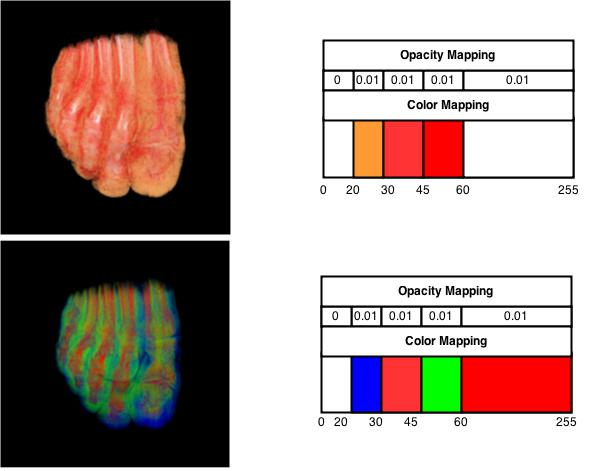
\includegraphics[width=350pt]{Images/foot_different_TF.jpg}
\caption{\label{fig:ray_cast1.jpg} Application of two different 1D transfer
functions on the same dataset. The transfer functions are shown next to their corresponding image.}
\end{figure} 


\subsection{Region of Interest}
A region of interest (often abbreviated ROI), is a selected subset of samples within a dataset identified for a particular purpose. A ROI can be any of the following.

\begin{itemize}
\item Volume of Interest, which is specified as a range of voxels within an 3D volume. For example, we could define a cubic, spherical or cylindrical ROI. 
\item A range of voxel intensities can also be a ROI.
\item A range of voxel intensities of one modality can be defined as an ROI in a multi-modal setup. 
\end{itemize}

\section{Volume Ray Casting}

Raycasting is a technique to visualize volume data. It is method in which for every pixel in the image, a ray is cast through the volume parallel to the view direction. The ray intersects(or passes close to) a line of voxels. The color of the pixel is computed based on color and transparency of the voxels that are intersected by the ray.

The ray equation is defined by a starting point and a direction, as shown in figure 2.2. If the ray hits the volume, the color of the pixel is calculated by sampling the data values of the ray at a finite number of positions in the volume. On each sample the transfer function is applied and composited with accumulated values of the ray.

\begin{figure}
\centering
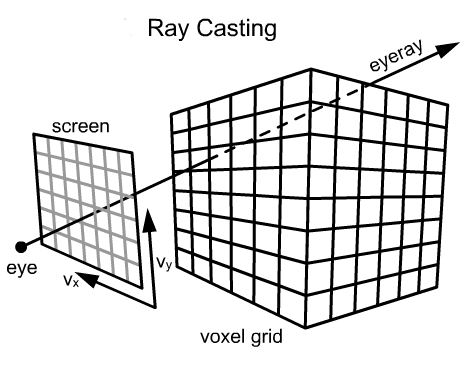
\includegraphics[width=220pt]{Images/ray_cast1.jpg}
\caption{\label{fig:ray_cast1.jpg} Direct volume rendering using raycasting.}
\end{figure}


\subsection{Basic Algorithm}

In its basic form, the volume ray casting algorithm comprises of a ray being cast through the volume, for each pixel of the final image. Generally, the volume is enclosed within a bounding primitive, a simple geometric object -- usually a cuboid -- that is used to intersect the ray of sight and the volume. Along the part of the ray of sight that lies within the volume, equidistant sampling points or samples are selected. In general, the volume is not aligned with the ray of sight, and sampling points will usually be located in between voxels. Because of that, it is necessary to interpolate the values of the samples from its surrounding voxels. After all sampling points have been fetched, they are composited along the ray of sight, resulting in the final color value for the pixel that is currently being processed. This compositing technique is explained in detail in a later section.

\subsection{Two-pass Rendering}

To perform raycasting on  a volume for an arbitrary view direction, we need to compute the points at which each ray enters and exits the cube corresponding to  the volume. An efficient and convenient method for this is to render the front and back faces of the cube into separate images, as shown in figure 2.4. The same pixel coordinates on the two images correspond to the images of points on a given ray, and specifically the entry and exit points of the ray. Thus, by tracking the mapping from points on the cube faces to the pixels on the images, we can compute the entry and exit point for each ray. \\



\begin{figure}
\centering
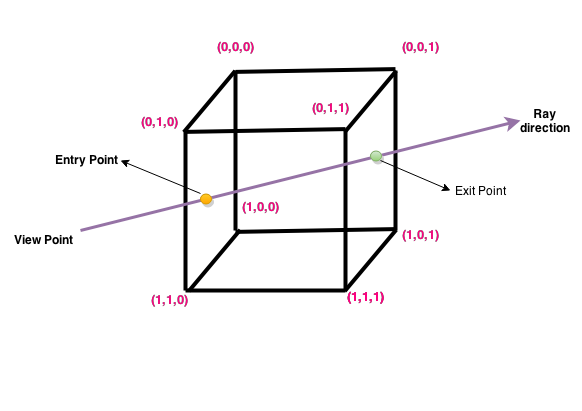
\includegraphics[width=320pt]{Images/cube.png}
\caption{\label{fig:ray_cast1.jpg} Assigning unique colors to all corners to the bounding box.}
\end{figure}


\lstdefinestyle{customc}{
  belowcaptionskip=1\baselineskip,
  breaklines=true,
  frame=L,
  xleftmargin=\parindent,
  language=C,
  showstringspaces=false,
  basicstyle=\footnotesize\ttfamily,
  keywordstyle=\bfseries\color{green!40!black},
  commentstyle=\itshape\color{purple!40!black},
  identifierstyle=\color{blue},
  stringstyle=\color{orange},
}


\lstset{style=customc}

\textbf{Pseudocode of Two-pass Volume ray casting:} 
\\
\begin{lstlisting}
First pass: render the backface of the boundbox  
Second pass: render the frontface of the boundbox
Lookup volume exit position from backface 2D texture 
Entry position obtained at second pass    
Compute ray of sight direction  

While in volume  
        Lookup data value at ray position  
        Apply transfer function to data value  
        Accumulate color and opacity  
        Advance along ray  
\end{lstlisting}	

We use two float-textures, where the color value encodes the co-ordinates of the entry and respectively the exit points. To obtain intersection of the ray of sight with data volume, we use a bounding box, which is a cube with each edge of unit length. Each of the eight corner vertex of the cube are assigned unique colors, as shown in figure 2.3. During rendering,  OpenGL will interpolate the color values between the vertices automatically. Since the corner colors are unique, we can use the interpolated colour values of a pixel to reconstruct the 3D coordinates of the intersection points of the ray of sight. On finding the entry and exit points on the cube, ray direction is easily obtained. From the entry point, ray starts marching towards the exit point while sampling points at equidistant locations.

\begin{figure}[!h]
\centering
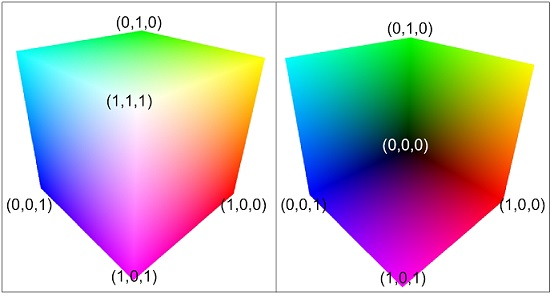
\includegraphics[width=350pt]{Images/ray_entry_exit.jpg}
\caption{\label{fig:ray_cast1.jpg} Entry and exit Textures.}
\end{figure}


\subsection{Sampling} 

Along the part of the ray of sight that lies within the volume, equidistant sampling points or samples are selected. In general, the volume is not aligned with the ray of sight, and sampling points will usually be located in between voxels, as shown in figure 2.5. Because of that, it is necessary to interpolate the values of the samples from its surrounding voxels. 

\begin{figure}[h]
\centering
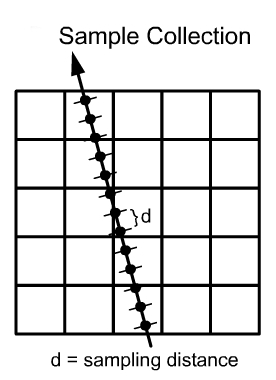
\includegraphics[width=120pt]{Images/sampling1.jpg}
\caption{\label{fig:ray_cast1.jpg} Sampling along the direction of ray.}
\end{figure}

\subsection{Compositing }

The discrete version of the volume rendering equation replaces the continuous integral with a Riemann sum. 

Discrete Volume Rendering Equations:

\begin{equation}
 C \; = \; \sum\limits_{i-1}^{n} \; C_i \; \prod\limits_{j=1}^{i-1} \; ( 1 \; - \; A_j) 
\end{equation}         
\begin{equation}
 A \; = 1 \; - \; \prod\limits_{j=1}^{n} \; ( 1 \; - \; A_j) 
\end{equation}

Here, Opacity $A_i$ approximates the absorption and opacity-weighted color $C_i$ approximates the emission and the absorption along the ray segment between samples i and i+1. 

This formula is efficiently evaluated by sorting the samples along the viewing ray and computing the accumulated color C and opacity A iteratively. The color of each sample is determined by classification and shading, and when the transparency is determined by classification, the next step is to evaluate the volume rendering equation using these values. This evaluation is performed by a process called compositing which generates the final pixel value for a ray shot into the volume. Two techniques for compositing  are front-to-back and back-to-front compositing.


\subsubsection{Back-to-Front Compositing Equations}

In this technique, samples are sorted in back-to-front order, and the accumulated color and opacity are computed iteratively. A single step of the compositing process is known as the Over Operator. 
 
\begin{equation}
\hat{C}_i \; = \; C_i \; + \; (1 \; - \; A_i ) \; \hat{C}_{i+1} 
\end{equation}
\begin{equation}
\hat{A}_i \; = \; A_i \; + \; (1 \; - \; A_i ) \; \hat{A}_{i+1} 
\end{equation}

where, ${C}_i$ and ${A}_i$ are the color and opacity obtained from the fragment shading stage for the ray i, along the viewing direction, and $\hat{C}_i$ is the accumulated color from the back of the volume.

\subsubsection{Front-to-Back Compositiong Equations}
In this technique, samples are sorted in front-to-back order. Front-to-back compositing has an added advantage over back-to-front compositing. Since the composition is done towards the back and the current transparency is known at all times, the compositing can be stopped early when the opacity is above a threshold (since nothing behind that point is going to affect the final image). This is one of the more powerful optimizations that can be done for several rendering techniques. \\

The front to back equation is:
\begin{equation}
\hat{C}_i \; = \; (1 \; - \; \hat{A}_{i-1} \; ) \; C_i \; + \; \hat{C}_{i-1}    
\end{equation}
\begin{equation}
\hat{A}_i \; = \; (1 \; - \; \hat{A}_{i-1} \; ) \; A_i \; + \; \hat{A}_{i-1}    
\end{equation}

where $\hat{C}_i \; and \; \hat{A}_i$ are the accumulated color and opacity from the front of the volume. 


\begin{figure}[h]
\centering
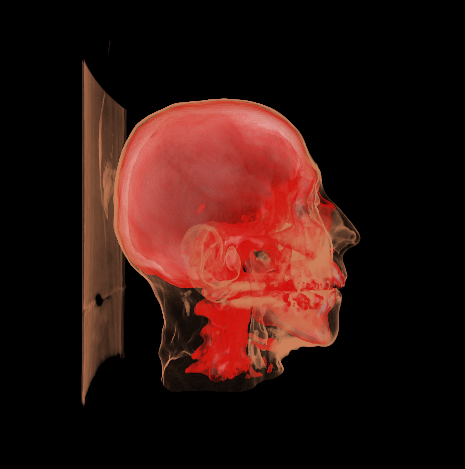
\includegraphics[width=220pt]{Images/dvr_head.png}
\caption{\label{fig:ray_cast1.jpg} Direct volume rendering of a volumetric head dataset.}
\end{figure}



% chap3.tex


\chapter{Visibility Driven Transfer function}\label{chap:ch4_abbr}

\section{Motivation}

Medical imaging has given radiologists an ability that photography was not able to provide, it lets them see inside the human body. With the advent of 3D visualization systems, these images can be put together into crisp and impressive renderings of the human body from a variety of perspectives that were only dreamt of before, revolutionizing clinical practice.

Light transport models soon emerged to allow light interactions that, although not realistic in the physical sense, proved to be more effective for understanding the complex relationships among the anatomical structures. For instance, bone could be made semi-transparent to provide visibility of brain tissue. Skin could be removed altogether from an image to show only muscle or internal organs. However, soon it
became evident that simply rendering these images in their raw form was no longer effective and the clear visualization of internal structures remains elusive.

The depiction of internal parts in the context of the enclosing space is a difficult problem that has occupied the mind of artists, illustrators and visualization practitioners. Despite the advances made in computer graphics for simulating the light transport in semi-transparent media, the problem of visualizing internal objects is no longer a rendering problem, but that of classification. Medical imaging technology obtains representations of anatomical structures via indirect ways, such as the response of tissue to X-rays or the alignment of electrons in a magnetic field. Therefore, the absence of semantic information prevents visualization practitioners from clearly marking up the regions that must be visualized. Without access to those regions, exploration becomes tedious and time-consuming. The predominant approach has been the use of transfer functions, or opacity mappings, which assign transparency properties to different intervals in the data. This method, however, does not guarantee visibility that internal structures or structures of interest in the volume. There is need to incorporate a measure for visibility. In this chapter, visualization techniques to obtain clear views of internal features in 3D volume data is discussed along with visibility metric.

\section{Related Work}

With the fast growth in computational power of graphics hardware, only until recently it has been possible to manipulate 3D volume data in fashions that were only possible for surface meshes and CAD models, where semantic information is often explicit and readily available. When volume data are understood as explorable objects, we can disassemble it into parts that can be decomposed in numerous ways. One of the foremost ideas that were explored in this direction where cutaways, where certain parts can be removed to uncover hidden parts of the 3D volume. [14] Exploded views extend this idea to reveal the relationships among the internal parts of a complex volume [1].

Another strategy is to assign material properties to different regions or layers of a volume and simulate the physical response to the deformation and cutting of such regions [5,6,10]. 

Although the deformation “unrealistically” simulates an elastic material for the piggy bank, the metaphor is effective for depicting the internal structures. More realistic effects are obtained by simulating the response of tissue, such as skin, to incisions and retractions, as used in real surgical procedures. Figure 3 shows the result of peeling the skin, and muscle layers of a foot CT scan to reveal the internal vessels (left) or bone (right).

Rigid and deformable cuts, although effective for visualizing the internal structures, work under the premise that the internal and external layers are clearly separated. In a more general sense, this separation is not easy to come by, and, in most cases, there is a degree of uncertainty. For this reason, the effective visualization of internal structure must rely on robust classification.

The main challenge when attempting to see the internal features remains that of classification. An effective visualization must first decide what is it that we must preserve and what regions are unimportant. Traditional classification systems, found in off-the-shelf visualization systems, only consider a single dimension for classification, without regards of the spatial characteristics or the semantics of the data. However, volume data seldom contain any semantics about the captured structures. Acquisition technology outputs a series of images with intensity values, while simulations of 3D phenomena sample a continuous scalar or vector field in a grid.

In an attempt to extract semantic information, one may analyze the spatial properties of the data, such as the location of boundaries [9], regions of high curvature [7], shape [12] or size[6]. In most of these cases, these properties are just approximations of the local distribution of data in a small neighborhood. Size, for example, can be measured as the extents of regions of a certain homogeneity. Regions of a certain material, such as brain, that occupy a large volume, have different properties than those regions, such as skull and
skin, that are relatively thin.

These observations have enabled us to construct classification based on size, and assign opacity based on the relative thickness of features. A particular example is the visualization of brain MRI, where the data is comprised of a series of thin layers (i.e, skin, skull and tissue) surrounding a large region, the brain, of a certain material. Exploiting these properties lets us minimize the effects of occluding tissue, such as skin, to reveal the brain tissue clearly, as shown in Figure 4.

Other approaches do not operate on the data itself but on the rendering process. For example, importance-driven techniques [13] and ghosted views [2,8] assign different opacities in a viewpoint dependent manner, so that the user constantly gets an uninterrupted view of internal structures. A different approach, opacity peeling, automatically finds the layers that compose an image from a given point of view [11].

\section{Notion of Visibility metric} 

One of the limitations of contemporary visualization systems is the inability to quantify how visible a feature of interest is. To be more effective, along with traditional transfer function design, must incorporate a measure of visibility. 

Visibility Metric attemps to measure the impact of individual samples on the image generated by a volumetric object. It is measured as the contribution of a structure of interest to the final image. Here, visibility can be used to quantify the quality of transfer function and ease their design towards more meaningful and efficient visualization. Transfer function generated with this approach are called as visibility driven transer functions.

This process measures visibility of all structures in a volume to arrive at a good transfer function. In general, a visibility-driven transfer function is constructed in such a way that we guarantee the visibility of all structures of interest and at the same time maximizes the visibility of structure of interest, in particular, of those features lying at the interior of a data set. 


\section{Visibility Histogram}

The contribution of a sample in the volume to final image is refered to as visibility of that sample. 


$ \alpha (s) \; = \; 1 \; - \; e^{\int^{D}_{s} \tau(t) dt \; } $   .....(3.1)


where $ \tau(t) $ is the attenuation coefficient of a sample, usually represented as an opacity transfer function $\mathcal{O}$ which is defined by user. Visibility also depends viewpoint as accumulated opacity in front of the sample may differ at different viewpoints. 

A visibility histogram is a graphical representation of distribution of visibility function in relation to the domain values of the volume. Samples are weighted by visibility and added into bins that partition the range of values in the scalar field. 

VH(x) = $ \mathcal{O} (x) \int_{s \epsilon \omega} \delta(s, x) (1 \; - \; \alpha(s) ) ds $  .....(3.2)
where, $ \delta(s, x) $ is a function.


\[
    \delta(s, x)=\left\{
                \begin{array}{ll}
                  1  \;\;\;\;\;\;\;    V(s) = x\\
                  0  \;\;\;\;\;\;\;    Otherwise \;\;\;\;\;\;\; .....(3.2)\\
                \end{array}
              \right.
\]



In this thesis, front-to-back compositing is used, as discussed in section 2.4.3. Accumulated opacity is computed as, 


AccumulatedOpacity[i] = AccumulatedOpacity[i-1] + ( 1 - AccumulatedOpacity ) Opacity(x) 

Hence, for all sample values x in the volume.
VH[x] = VH[x] + ( 1 - AccumulatedOpacity ) Opacity(x)

\begin{figure}
\centering
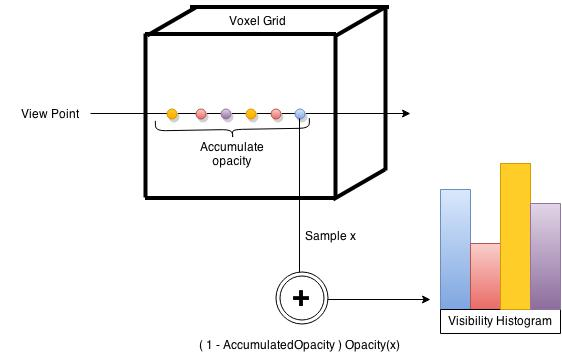
\includegraphics[width=350pt]{Images/VHistogram.jpg}
\caption{\label{fig:ray_cast1.jpg} Direct Volume rendering using Raycasting.}
\end{figure}


Visibility histogram helps find string occusion patterns on the data, as shown in the figure 3.1. 


\begin{figure}
\centering
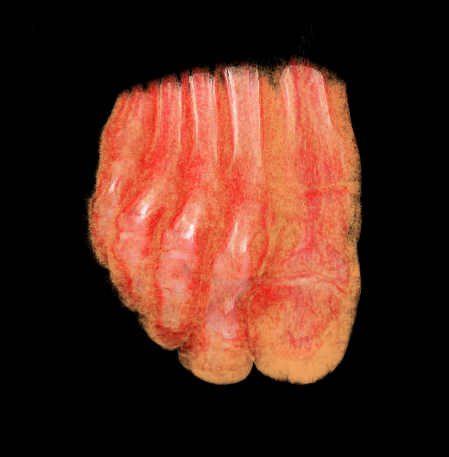
\includegraphics[width=150pt]{Images/foot_1.png}
\caption{\label{fig:ray_cast1.jpg} Direct Volume rendering using Raycasting.}
\end{figure}






   


% chap4.tex 


\chapter{Visibility guided multimodal volume visualization }\label{chap:errors}


\section{Motivation }

It is often desirable to visualize multimodal data by rendering the multiple volumes into one image. The general approach to this visualization is to fuse the multiple datasets based on their weighted intensity values. For example, CT is usually used to give us contextual information, to show anatomical relationship between pathological tissue (highlighted with PET data) and other non-effective regions. However with this approach, the intensity of the target area is often similar to that of neighbourhood resulting in lack of focus and clarity of sections of interest.  Another approach when intensities are similar, is to manually segment out a part, and define a separate transfer function for highlighting the target area. Such manual tasks are tedious and error-prone.  

\section{Context+Focus Visualization For Multimodal Volume}

The advantage of using additional modalities is that they provide complementary or supplementary information. However, handling of multiple sources for a structure, and generating a single image from them, is quite challenging.  
 
The notion of visibility, as discussed in the previous chapter, helps us to summarize distribution for visibility a structure of interest from a given viewpoint. For example PET and CT dataset, PET data acts as the ROI we need to focus and CT data gives us the context. The techniques discussed in the previous chapter can used to modulate CT data opacities to obtain "focus+context" visualization. 

\section{Local Visibility Histogram}

One technical challenge that lies in multimodal dataset visualization is in ROI definition. One way would be set up a ROI around the structure of interest manually by identifying some key boundary points. If the structure is complex, user needs to define a larger number of boundary points around the ROI, which is time-consuming and error-prone. One solution to this problem is to define a sphere or bounding box covering the ROI, as shown in figure 4.1. This solution is difficult to adopt, when the structure is complex, scattered or noisy. 


\begin{figure}[!h]
\centering
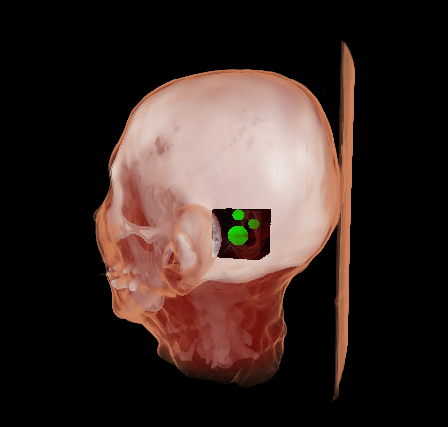
\includegraphics[width=350pt]{Images/Vol-ROI.png}
\caption{\label{fig:ray_cast1.jpg} ROI bounded by a volume.}
\end{figure}

One approach to increase visibility of ROI is to make occluding materials completely transparent, but this completely loses all the context information. Hence, for those rays hitting the ROI, local histograms is computed for each ray, as shown in figure 4.2. Rest of the rays cast into the volume are used to compute the global histogram. Using this, the user will now be able to manipulate the area of ROI, and control the visibility of this area. Upon varying the view direction local histogram is recalucated. 


\begin{figure}[!h]
\centering
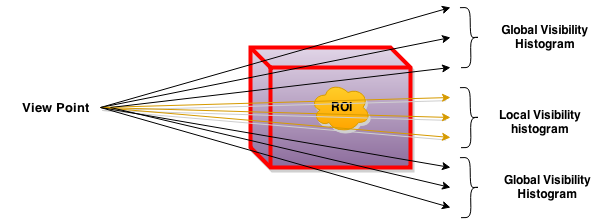
\includegraphics[width=300pt]{Images/pet-ct-roi.png}
\caption{\label{fig:ray_cast1.jpg} Global histogram and local histogram.}
\end{figure}
 

Once visibility histogram is known, opacity of samples in the ROI are adjusted using the formula 4.1.

\begin{equation} 
A^{'}(x) \; = \; A(x) \; ( \; 1 \; - \; VH(X) \; )^{e} 
\end{equation}

where, A($x$) and A$^{'}(x)$ are the old and new opacity mappings for intensity $x$. VH($x$) is the visibility associated with that intensity in the visibility histogram. $e$ is the exponent that defines the strength of such a mapping, as illustrated in the figure 4.3.

From equation 4.1, when VH($x$) is high(ie., it is more visible) it is likely to be made more transparent. When VH(x) is low, these samples do not occlude much and are retained to provide context. This helps in keeping context clear which increasing the focus. 


\begin{figure}[ht]
\centering
%\begin{minipage}[b]{0.45\linewidth}
e = 0    \hspace{140pt}      e = 1 \\
\vspace{3pt}
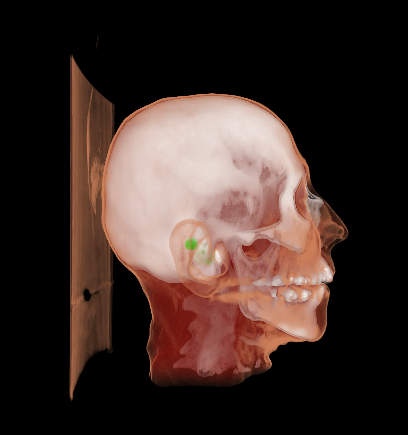
\includegraphics[width=150pt,height=150pt]{Images/i=0.png}
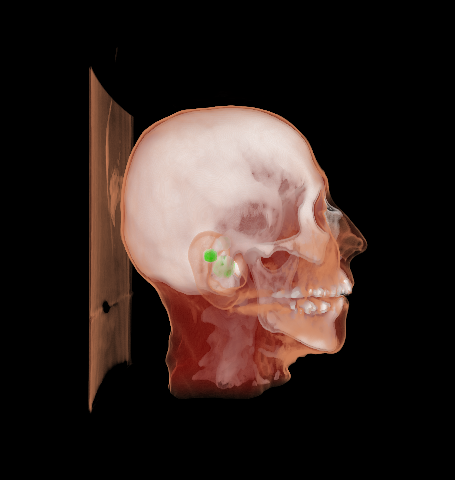
\includegraphics[width=150pt,height=150pt]{Images/i=1.png}\\
e = 3    \hspace{140pt}      e = 10 \\
\vspace{3pt}
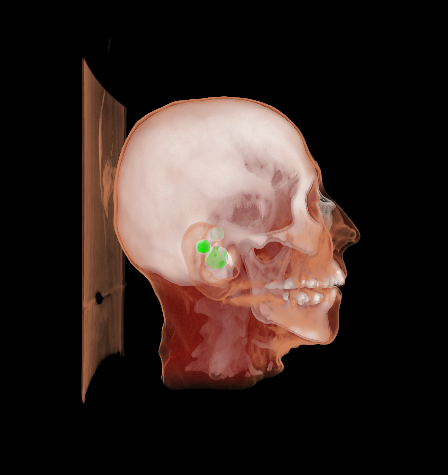
\includegraphics[width=150pt,height=150pt]{Images/i=3.png}
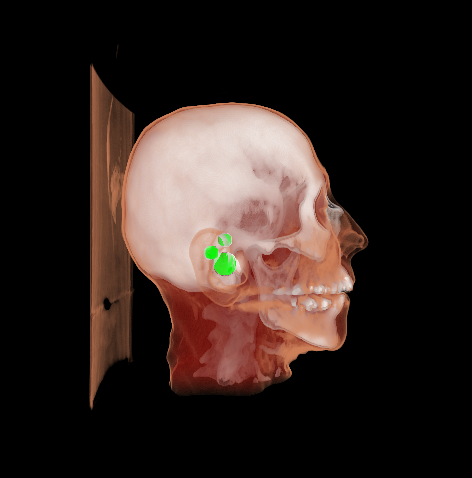
\includegraphics[width=150pt,height=150pt]{Images/i=10.png}
\caption{Effects of visibility-weighted adjustment $e$. }
\end{figure}




% chap5.tex

\newcommand{\BibTeX}{Bib\TeX}

\chapter{Handling Citations}\label{chap:refs}

\BibTeX{} can be used to handle all your bibliographic needs.  Simply add
references to the file \texttt{ref.bib} and \BibTeX\ will take care of
the rest.  An example of a \BibTeX{} book, conference paper and journal
article are given in the sample \texttt{ref.bib} file.  Many online
journals have links to \BibTeX{} citations that you can download and
incorporate into the \texttt{ref.bib} file. {\it Do not change the name of
  the file} \texttt{ref.bib}.

The order of the fields is unimportant. \BibTeX\ will display them
in the correct order when constructing your bibliography.  Also note
that you can specify information about a reference that may not even be
included in the actual bibliography.  For example, the ISBN field is not
required by the bibliography, but you can, if you want, put the ISBN to
the \BibTeX{} entry.

We can cite a journal article~\cite{someguy2002} and a conference
paper~\cite{LastName1996} in the same way as a book citation.  More
information can be found in~\cite{lam1994}.

% chap6.tex

\chapter{Results}\label{chap:}

We applied our approach discussed in the thesis to a number of datasets, both medical and non-medical. We have shown that use of visibility histogram alone prove to be an important element towards the understanding of complex datasets. A key point of our work to demonstrate visibility histogram are a useful aid to quantify the information derived from the structure of interest in both single and multimodality setup. Results show it helps user generate desired visualization, by intuitively designing the transfer function, and thus enabling user to gain insights into the volume. Our technique of two-pass volume raycasting, which is implemented on GPU shaders, has lead to improved performance with better user experience. Thereby meeting the objective of this thesis. To validate our work, we plan to demonstrate our solution to radiologists and get them to evaluate our work based on the parameters of usability, performance and correctness of the solution.   

Although the objectives of this thesis have been satisfied, we consider that the work can be extended in different ways. As part of future work, we can incorporate lighting for better illustrative visualization. We can extend to two-dimensional transfer functions, for silhouette rendering in ROI and produce enhanced visualizations by incorporating NPR techniques. Volume raycasting and visibility driven transfer function techniques can also be used to visualize iso-surfaces of volumetric dataset. Another important future work is to extent our work to enable visualization of non-uniform grids. We can also extend our approach to study effects of intergrating other NPR technique for multimodal visualization. We can work on the implementational aspects of the semi-automatic transfer function generation.


 




\setbib

% If you have no appendices, remove the following three lines.
% If you have more appdences, add them as necessary.
\appendix
% apdxa.tex

\chapter{Appendix: How to Add an Appendix}\label{apdx:a}

This is Appendix~\ref{apdx:a}.

You can have additional appendices too, (\emph{e.g.}, \texttt{apdxb.tex},
\texttt{apdxc.tex}, \emph{etc.}). These files need to be included in
\texttt{thesis.tex}.

If you don't need any appendices, delete the appendix
related lines from \texttt{thesis.tex}.

% apdxb.tex

\chapter{Appendix: How to Add Another One}\label{apdx:b}

This is Appendix~\ref{apdx:b}.


\end{document}
